%%%%%%%%%%%%%%%%%%%%%%%%%%%%%%%%%%%%%%%%%%photos,%%%%%%%%%%%%%%%%%suggested.%%%%%%%%%%%%%%%%%%%%%%%%%%%%%%%%%%%%%%%%%
%%%%%%%%%%%%%%%%%%%%%%%%%%%%%%%%%%%%%%%%%%%%%%%%%%%%%%%%%%%%%%%%%%%%%%%%%%%%%%%%%%%%%%%%%%%%%%%%%%%%%%%%%%%%%%%%%%%%
%%% ARTICLE
%%%%%%%%%%%%%%%%%%Recall%%%%%%%%%%%%%%%%%%%%%%%%%%%%%%%%%%%%%%%%%%%%%%%%%%%%%%%%%%%%%%%%%%%%%%%%%%%%%%%%%%%%%%%%%%
%%%%%%%%%%%%%%%%%%%%%%%%%%%%%%%%%%%%%%%%%%%%%%%%%%%%%%%%%%%%%%%%%%%%%%%%%%%%%%%%%%%%%%%%%%%%%%%%%%%%%%%%%%%%%%%%%%%%
%\clearpage % It is recommended to leave only the abstract data on the first page, although this is not mandatory.

\section{Introduction}

This model instruction text has been developed so that authors can present their articles in a standardized way.
It has been adapted from the template of the \href{https://revista.acustica.org.br}{Acoustics and Vibrations Journal}, for use in the XIII~Ibero-American Congress on Acoustics (FIA 2024).
%
This will provide uniform formatting for the full articles of the event.
This template presents the main guidelines for preparing a complete article in terms of content presentation, graphics, structure, layout, and the procedure for article submission. 
%
This document already includes custom style formatting to help draft the article. Therefore, the author can use this file as a template for this purpose. The templates will be available in Microsoft Word (\texttt{.docx}) and \LaTeX\xspace (\texttt{.tex}). This version is also available on \href{https://www.overleaf.com/read/tjbcfwbtfdtz\#869489}{Overleaf} and \href{https://github.com/willdfonseca/latex}{GitHub} --- and is compatible with Windows, Mac, and Linux. 
%
The authors are responsible for the content, preparation, and submission of the articles according to this template.

The complete text should be single-spaced, using Times New Roman font size 12~pt, and paragraphs with 0~pt spacing before and 6~pt after. It is common practice to write scientific articles in an impersonal tone, so this is recommended. In addition, the articles will be accepted in formal Portuguese, English\footnote{Non-native speakers writing in a foreign language should preferably have their work professionally reviewed.}, and Spanish\footnotemark[2]. 

%%%%%%%%%%%%%%%%%%%%%%%%%%%%%%%%%%%%%%%%%%%%%%%%%%%%%%%%%%%%%%%%%%%%%%%%%%%%%%%%%%%%%%%%%%%%%%%%%%%%%%%%%%%%%%%%%%%
%%%%%%%%%%%%%%%%%%%%%%%%%%%%%%%%%%%%%%%%%%%%%%%%%%%%%%%%%%%%%%%%%%%%%%%%%%%%%%%%%%%%%%%%%%%%%%%%%%%%%%%%%%%%%%%%%%%
\section{Basic guidelines}

This section provides a summary of how the article should be constructed. For more details, refer to the subsequent sections.

\vspace{-8pt}
\begin{enumerate} \itemsep=2pt
    \item The provided LaTeX and Word templates already contain all the configurations described in this document. Additionally, this manuscript provides simultaneous instructions for both text layout platforms.
	\item The first page should contain (for Portuguese and Spanish languages) title, authors, affiliations, abstract, keywords, --- and in English --- \textit{title}, \textit{abstract}, and \textit{keywords}. Submissions in English may contain only authors, affiliations, \textit{title}, \textit{abstract}, and \textit{keywords} (without versions in Portuguese or Spanish).
	\item The text must be written in formal language.
	\item The number of pages must be a minimum of 6 and a maximum of 15, counting from the title page to the end of the references (including appendices, if any).
	\item The paper size is A4, with margins: top 2.0~cm, bottom 2.0~cm, left 1.8~cm, and right 1.8~cm (the spacing between columns is 1.0~cm).
	\item The text should be written in Times New Roman font size 12~pt (as per this template).
	\item The article may contain figures, tables, codes, and equations. If necessary, links may be included in the text. Animations are also accepted, provided they are formatted as figures.
	\item A technical article is understood to have a logical structure, descriptive content, and reproducible results, concluding with references.
\end{enumerate}

%%%%%%%%%%%%%%%%%%%%%%%%%%%%%%%%%%%%%%%%%%%%%%%%%%%%%%%%%%%%%%%%%%%%%%%%%%%%%%%%%%%%%%%%%%%%%%%%%%%%%%%%%%%%%%%%%%%
%%%%%%%%%%%%%%%%%%%%%%%%%%%%%%%%%%%%%%%%%%%%%%%%%%%%%%%%%%%%%%%%%%%%%%%%%%%%%%%%%%%%%%%%%%%%%%%%%%%%%%%%%%%%%%%%%%%
\section{Document and presentation}

Always place text in sections and subsections, do not leave them orphaned (opening a section and proceeding directly to the subsection).

%%%%%%%%%%%%%%%%%%%%%%%%%%%%%%%%%%%%%%%%%%%%%%%%%%%%%%%%%%%%%%%%%%%%%%%%%%%%%%%%%%%%%%%%%%%%%%%%%%%%%%%%%%%%%%%%%%%
\subsection{First page}

The first page should contain the following items provided by the authors: title, authors, affiliations, abstract, keywords, \textit{title}, \textit{abstract}, and \textit{keywords}. 
%
If the complete title is very long, a shorter version is requested to be included in the article's header.

The abstract of the article should be between 150 and 200 words (in 11~pt font). The abstract, keywords, \textit{title}, \textit{abstract}, and \textit{keywords} make up the first page of the article, and it is recommended not to extend to the second page. 
It should provide a concise presentation of the scientific technical article, including an introduction, the objective, a summary of the methodology, the main result, and the main conclusion (preferably in that order). It is not necessary to separate it into items or sections within the abstract. In this way, the reader can grasp the essence of the work. Recall that the abstract is like a movie trailer; people will be interested in reading the entire article if the abstract catches their attention. The abstract should not contain new information not included in the article; undefined abbreviations; prior discussion of other literature; references and citations; and excessive details about the methods used. It is also not the introductory paragraph of the document, which should be placed at the beginning of the text. Use only useful and relevant information, and practice empathy with the potential interested reader. To obtain a cohesive, elegant abstract that aligns with the article, write a draft, complete the document, and, at the end, review it to ensure the content consistently reflects the document's essence. 

Following the abstract, the author should list up to five keywords (avoid using the same words that form the article title). The text of the article should start properly after the \textit{keywords}.

In the authors' affiliations, use numbers as markers, and if there are authors from the same institution, use only one address, and differentiate them by emails. When there are emails from the same domain, try to reduce them using braces \{\}. Use a maximum of two lines for the affiliation of each author from different institutions. See some examples below.
%
\begin{flushleft}
\vspace{-0.25\baselineskip}
\begin{itemize}[topsep=-1ex,align=left,leftmargin=0.2cm] \itemsep=4pt

	\item Fonseca,~W.~D'A.$^1$; Surname,~N.$^2$\\[6pt]	
	$^{1,\,2}$\,Acoustical Engineering Program, Federal University of Santa Maria, Santa Maria, RS, Brazil, 
	 will.fonseca@eac.ufsm.br, name@domain.br.
	
	\item Fonseca,~W.~D'A.$^1$; Mareze,~P.~H.$^2$\\[6pt]	
	$^{1-2}$\,Acoustical Engineering Program, Federal University of Santa Maria, Santa Maria, RS, Brazil,\\
	\{will.fonseca, paulo.mareze\}@eac.ufsm.br.
	
	\item Fonseca,~W.~D'A.$^1$; Surname,~N.$^2$, Mareze,~P.~H.$^3$\\[6pt]	
	$^{1,\,3,\,2}$\,Acoustical Engineering Program, Federal University of Santa Maria, Santa Maria, RS, Brazil,\\
	\{will.fonseca, paulo.mareze\}@eac.ufsm.br, name@domain.br.

	\item Fonseca,~W.~D'A.$^1$; Surname,~N.$^2$\\[6pt]	
	$^{1}$\,Acousticap Engineering Program, Federal University of Santa Maria, Santa Maria, RS, Brazil,
	will.fonseca@eac.ufsm.br.\\[4pt]		
	$^2$\,Laboratory, Institution, City, State, Country, name@domain.br.	
\end{itemize}
\vspace{-0.4\baselineskip}
\end{flushleft}

%%%%%%%%%%%%%%%%%%%%%%%%%%%%%%%%%%%%%%%%%%%%%%%%%%%%%%%%%%%%%%%%%%%%%%%%%%%%%%%%%%%%%%%%%%%%%%%%%%%%%%%%%%%%%%%%%%%
\subsection{Number of pages}

The complete work should contain 6 to 15 pages, counting from the title page to the end of the reference list. Appendices are allowed after the references, provided that they do not exceed 15 pages in total.

To maximize the content on each page, figures, tables, and codes should be presented throughout the body of the text (side-by-side figures are accepted).

%%%%%%%%%%%%%%%%%%%%%%%%%%%%%%%%%%%%%%%%%%%%%%%%%%%%%%%%%%%%%%%%%%%%%%%%%%%%%%%%%%%%%%%%%%%%%%%%%%%%%%%%%%%%%%%%%%%
\subsubsection{Example of a two-level subsection}

This is a two-level subsection for exemplification purposes.

%%%%%%%%%%%%%%%%%%%%%%%%%%%%%%%%%%%%%%%%%%%%%%%%%%%%%%%%%%%%%%%%%%%%%%%%%%%%%%%%%%%%%%%%%%%%%%%%%%%%%%%%%%%%%%%%%%%
\subsection{Page size and margins}

The text should be configured on A4 size paper (210~mm $\times$ 297~mm), in a single column, with distinct numbering for even and odd pages (as in this document). The left and right margins should be 1.8~cm, the bottom 2.0~cm, and the top 2.0~cm. Try to utilize the entire available area. Exceptions can be made, for example, when it is necessary to start a new section, title, subtitle, or caption; these may be allocated at the beginning of the next page.

%%%%%%%%%%%%%%%%%%%%%%%%%%%%%%%%%%%%%%%%%%%%%%%%%%%%%%%%%%%%%%%%%%%%%%%%%%%%%%%%%%%%%%%%%%%%%%%%%%%%%%%%%%%%%%%%%%%
\subsection{Characters and text}

The texts should be written in Times New Roman font. The article title should be on the first page, centered, \textbf{bold}, with only the first letter capitalized (except for proper names), in 18~pt font, and a paragraph spacing of 22~pt afterward. Section titles should be in bold, 12~pt font, with only the first letter capitalized (unless there are proper names), as shown in this template. The subsections should also be in bold, 12~pt font; for both cases, use Times New Roman font. The document text should be single-spaced, 12~pt font, justified, and without indentation in the first line. Avoid using subsections with more than three levels and instead use a list system.

% In LaTeX this is already configured automatically.

Use formal and scientific language in your text\footnote{Footnotes can help clarify details and comments.}. Foreign words should be italicized (for example, as in \textit{instrumentação}). Acronyms, abbreviations, and/or other constructions that are not common knowledge should be explained to the reader, for example, HRTF (\textit{Head-Related Transfer Function}) --- always written upright, including in equations.
Conduct technical and grammatical reviews before submission.

%%%%%%%%%%%%%%%%%%%%%%%%%%%%%%%%%%%%%%%%%%%%%%%%%%%%%%%%%%%%%%%%%%%%%%%%%%%%%%%%%%%%%%%%%%%%%%%%%%%%%%%%%%%%%%%%%%%
\subsection{Line and paragraph spacing}

Single line spacing should be used, as already adopted in this instruction file. For paragraph formatting, choose the justified paragraph option (with 6~pt spacing).

% In LaTeX this is already configured automatically.

%%%%%%%%%%%%%%%%%%%%%%%%%%%%%%%%%%%%%%%%%%%%%%%%%%%%%%%%%%%%%%%%%%%%%%%%%%%%%%%%%%%%%%%%%%%%%%%%%%%%%%%%%%%%%%%%%%%
\subsection{Equations and units}

Units from the International System (SI) will be adopted. When writing your work in Portuguese or Spanish, \textbf{use the comma as the decimal separator} (according to the current Portuguese and Spanish languages), whether in text, tables, figures, and/or graphs. Always strive for consistent precision when comparing numbers, for example: 3.0 is different from 3.00, but has the same precision as 6.0.
If the work is written in English, it is up to the author to use either a period or a comma as the decimal separator (as long as the notations are not mixed).
When writing a number with its unit\footnote{Units are always written ``upright'', i.e., not in italics, for example, 30~N/m$^2$.}, always keep the number together with the corresponding unit, without a line break between them (in MS Word, use Ctrl + Shift + Space [or Alt + 0160], in \LaTeX\xspace use a tilde ($\sim$) between the number and the unit). For example, 3~m separates the input and output and 4,512.28~cm is the measured distance.

Equations should be integrated into the text (in Word, use a simple ``table'') as in the example of Equation~\eqref{eq:area-circ}. They should also be centered and numbered sequentially, with the numbering placed on the right side and in parentheses (see the example). Recall that they are textual elements, so they should be punctuated, and the following text should not normally start with a capital letter. It is recommended to place the nomenclature immediately after the presented variable.

The area of the circle (in m$^2$) is given by
%
\begin{equation}
	A = \pi \, r^2\;,
\label{eq:area-circ}
\end{equation}
%
where $r$ is the radius in meters (m). Remember that variables (like $r$ in this example) are written in \textit{italics} (whether in the equation or the text). However, \textbf{units, functions, and mathematical operators are written ``upright''}, without italics. For example, 32.0~N/m$^2$ was the applied pressure, or
%
\begin{equation}
	\int_a^b p(\phi)\, \dt p\,
\label{eq:int}
\end{equation}
%
was the calculated integral (note that the differential operator ``d'' is upright), for each angle $\phi$ in degrees. Examples of functions include sine, $\sin(\theta)$, or $\log(y)$.

Subscript and superscript text will be in italics only if it corresponds to a relevant variable. If it is a ``complementary name'', the text should be upright, for example, $P\txu{total}$ corresponds to the total pressure in Pa, or $S\txup{tri}$ corresponds to the triangle area in cm$^2$. 
%
However, when referring to a variable, such as $i$, one should write, for example: ``the summation was calculated considering $P_i$ up to the final $i$-th pressure, corresponding to 256''.

If text, acronyms, or units are used in equations, they should be represented upright, for example:
%
\begin{equation}
	\text{density} = \frac{\tx{mass}}{\;\;\tx{volume}\;\;}\,,
\label{eq:density}
\end{equation}
%
where in SI (International System of Units), the unit of density is kilogram per cubic meter (kg/m$^3$).
%
In the text, when it is necessary to cite a previously presented equation, it should be done as follows: Equation~\eqref{eq:density} — with only the first letter capitalized and the corresponding number in parentheses.

%%%%%%%%%%%%%%%%%%%%%%%%%%%%%%%%%%%%%%%%%%%%%%%%%%%%%%%%%%%%%%%%%%%%%%%%%%%%%%%%%%%%%%%%%%%%%%%%%%%%%%%%%%%%%%%%%%%
\subsection{Figures, tables, and codes}

Figures and tables should be inserted within the text, preferably following the paragraphs to which they refer. A mention of figures, tables, and codes in the running text before their presentation is necessary to guide the reader. Figures and tables must contain all the formatting and content elements so that they can be interpreted correctly, without having to resort to the running text to find additional information.  Tables and figures should be separated from the text with \textbf{one (1) blank line} before and after (12~pt).

% In LaTeX this is already configured automatically.

Figures, tables, and codes\footnote{The distribution of this \LaTeX\xspace template includes the \ttc{Codes2Latex.sty} package, which enables possibilities for documenting generic codes and languages such as Matlab, Fortran, Python, LabView, and LaTeX in an organized manner (see Code~\ref{code.matlalatex}) --- the package is still under development.} should be centered and numbered sequentially (see the examples in Figures~\ref{fig:beamforming} and \ref{subfig.exemplo}; Tables~\ref{tab.exemplo} and \ref{quad.exemplo}; and Code~\ref{code.matlalatex}). Strive to use figures and graphs that are entirely comprehensible.

The label and number of the figures, followed by the caption, should appear immediately below and centered (10~pt). If using figures from other authors (or sources), even if adapted, indicate the source immediately after the descriptive caption, as shown in Figure~\ref{fig:beamforming}.

The label, number, and caption of the tables and codes should appear centered at the top (see Table~\ref{tab.exemplo}). The source of the tables should be presented according to the original publication (when necessary). Table~\ref{tab.exemplo} provides an example of the style to be used (the table content may have a smaller font size than the text when necessary). Additionally, the automated cross-referencing system is strongly recommended. \textbf{Remember that all objects, such as figures and tables, must be cited in the text.}

It is recommended that graphics, figures, photos, and any other graphic files are inserted in the text in .jpg and/or .png format with good/adequate quality (or in vector format in .pdf for \LaTeX\xspace users). Make sure that the graphics and pictures are legible (especially if the information is relevant).

\begin{figure}[!ht] %% Example of a figure
	\centering
	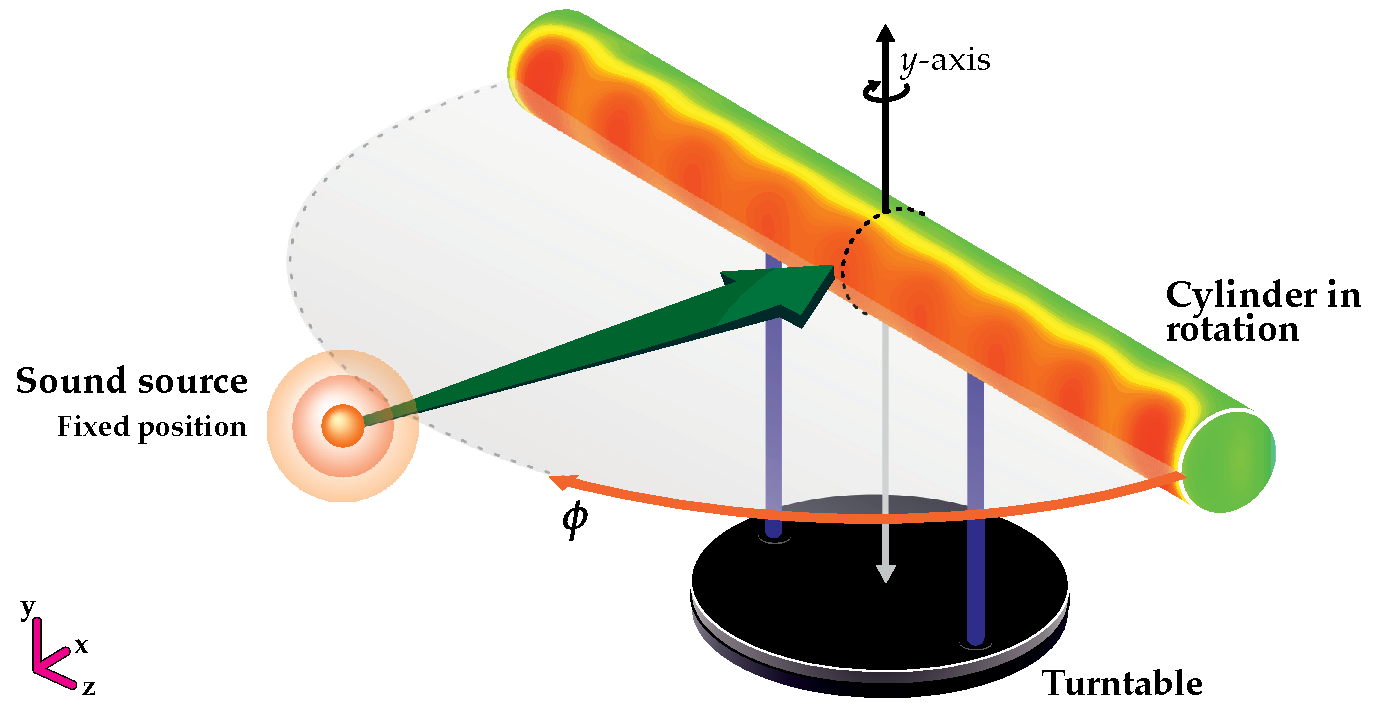
\includegraphics[width=0.70\linewidth]{figs/Measurement-Scheme-Fonseca-2013-en.pdf}%
	\caption{Beamforming measurement with cylindrical array (adapted from Fonseca \cite{Fonseca-2013}) — example of a figure.}
	\label{fig:beamforming}%
\end{figure}

\begin{figure}[!ht]
  %\ContinuedFloat %% to continue from the previous figure
  \centering
	\subfloat[Caption for Figure~\protect\subref*{fig.figA}.]{\label{fig.figA}
            \makebox[.46\columnwidth]{\includegraphics[height=35mm,page=48]{example-image-duck}} } % makebox helps organize side-by-side figures
	\quad
  \subfloat[Caption for Figure~\protect\subref*{fig.figB}.]{\label{fig.figB}
            \makebox[.46\columnwidth]{\includegraphics[height=35mm,page=47]{example-image-duck}} }
  \caption{Example of side-by-side figures.}
  \label{subfig.exemplo}
\end{figure}


\begin{table}[ht!]
%\vspace{-2mm}
  \centering \ratb{1.3} \setlength\aboverulesep{0pt} \setlength\belowrulesep{0pt}
  \caption{This is an example of a table.}
    \fontsize{11}{12}\selectfont 
    \begin{tabular}{| C{2.8cm} | C{1.8cm} | C{1.8cm} |}
    \hline
	\SetRowColor{LightBlue}
    \textbf{ Experiment / Type } & \textbf{Exp. 1} & \textbf{Exp. 2}\\
	\midrule
		Type 1 & Green & Yellow\\
		\rowcolor[gray]{.95} Type 2 & Blue & White\\
	\hline
    \end{tabular}
    \label{quad.exemplo}%
    \vspace{2mm}
\end{table}%

\begin{table}[!htb]
  \centering \ratb{1.3} 
  \caption{Microgeometric and macroscopic properties of porous layers CPA 1 and CAUQ-B\\ (extracted from Mareze \etal \cite{Mareze-2017}) --- example of a table.}
	\fontsize{11}{12}\selectfont 
    \begin{tabular}{C{2.9cm} | C{1.5cm} | C{1.5cm} | C{1.5cm} | C{1.5cm} | C{1.5cm} | C{1.0cm}| C{1.0cm}}
    \toprule
		\SetRowColor{LightOrange}
    \textbf{ Sample / Parameter } & $L\txu{p}$ \qquad [$\upmu$\! m] & $L\txu{a}$ \qquad [$\upmu$\! m] & $D\txu{p}$ \qquad [$\upmu$\! m] & $D\txu{a}$ \qquad [$\upmu$\! m] & $\sigma$ [Ns/m\txup{4}] & {$\phi$\quad [--]} & $\alpha_{\infty}$ [--]\\
	  \midrule
		CPA 1 $\Rightarrow$  3.0\% &	1359.81 & 1492.51 & 2344.05 & 1425.67 &	5131 &	0.218 &	1.63\\
		\rowcolor[gray]{.95} CAUQ-B $\Rightarrow$ 4.5\%	& 1598.29 &	701.24 & 2126.46 & 895.34 &	54989 &	0.070 &	2.89\\
    \bottomrule
    \end{tabular}
    \label{tab.exemplo}%
\end{table}%

%% Example of side-by-side figures using minipage
%\begin{figure}[!htb]
    %\centering
    %\begin{minipage}[t]{.48\textwidth}
        %\centering
        %
\includegraphics[width=1\linewidth,page=2]{FIA-logo.pdf}
        %\caption{Left side figure.}
        %\label{fig:ladoE}
    %\end{minipage}%
		%\quad
    %\begin{minipage}[t]{0.48\textwidth}
        %\centering
        %
\includegraphics[width=1\linewidth,page=2]{FIA-logo.pdf}
        %\caption{Right side figure.}
        %\label{fig:ladoD}
    %\end{minipage}
%\end{figure}

\begin{matlabcode}[Example of a code snippet (making Matlab write LaTeX).]{code.matlalatex}
  syms x
  f = taylor(log(1+x));
  latex(f)
\end{matlabcode}

All elements (such as figures and graphs) can be in color or grayscale. Avoid using textual elements from other authors without proper citation (and/or authorization). Figures containing text are essential to be in the same language as the article. Avoid indirect citations such as \textit{Google Images}, and avoid using volatile knowledge bases.

Cross-references should be made for all elements, for example: Figure~\ref{fig:beamforming} and Table~\ref{tab.exemplo} (with only the first letter capitalized, avoid line breaks between the label and the respective number). If there is a subfigure, use Figure~\subref*{fig.figA}, for example.


%%%%%%%%%%%%%%%%%%%%%%%%%%%%%%%%%%%%%%%%%%%%%%%%%%%%%%%%%%%%%%%%%%%%%%%%%%%%%%%%%%%%%%%%%%%%%%%%%%%%%%%%%%%%%%%%%%%
\section{Types of articles}

The event will accept \textbf{original submissions} (i.e., not yet published) of scientific research and applications in engineering, architecture, audio, physics, mathematics, speech therapy, and related areas (and subareas). Thus, the following types of documents are suggested:
%
\begin{itemize}[topsep=0ex] \itemsep=2pt
	\item \textbf{Technical and applied papers}:
	present original material from applications of known and/or developing techniques. They should describe applied methods that comply with standards and/or present relevant results. It is essential that these articles interest researchers and professionals in the proposed area.
	
	\item \textbf{Scientific papers}: 
	include original (ideas, models, experiments, \etc) unpublished material that significantly contributes to the advancement of scientific knowledge in the addressed topic. The content should establish a connection with the existing state-of-the-art in the published literature.

	\item \textbf{Review papers}:
	discuss the state-of-the-art on the subject in question, elucidating from basic concepts to more complex aspects. This type of submission should be comprehensive regarding the existing literature, broadly covering ideas, models, experiments, \etc, already developed, even if they disagree with the author's view. It is crucial that the topic is of interest to the scientific community.
\end{itemize}

\vspace{5pt}

The thematic areas of the event include:
%	
\begin{enumerate}[topsep=0ex] \itemsep=0.0pt
    \item Acoustics Education
    \item Architectural and Building Acoustics
    \item Biomedical Acoustics and Bioacoustics
    \item Computational Acoustics
		\vspace{-0.25em}
    \begin{enumerate}[noitemsep,topsep=0ex] 
        \item Acoustic Imaging and Virtual Acoustics/Auralization
    \end{enumerate}
    \item Environmental, Industrial, and Occupational Noise
    \item Forensic Acoustics
    \item Musical Acoustics
    \item Physical Acoustics and Ultrasound
		\vspace{-0.25em}
    \begin{enumerate}[noitemsep,topsep=0ex]
        \item Structured Metamaterials for Noise and Vibration Control
    \end{enumerate}
    \item Professional Audio and Electroacoustics
    \item Psychological and Physiological Acoustics
    \item Signal Processing in Acoustics
    \item Soundscapes and Ecoacoustics
    \item Structural Acoustics and Vibrations
    \item Underwater Acoustics
\end{enumerate}

	
%%%%%%%%%%%%%%%%%%%%%%%%%%%%%%%%%%%%%%%%%%%%%%%%%%%%%%%%%%%%%%%%%%%%%%%%%%%%%%%%%%%%%%%%%%%%%%%%%%%%%%%%%%%%%%%%%%%
%%%%%%%%%%%%%%%%%%%%%%%%%%%%%%%%%%%%%%%%%%%%%%%%%%%%%%%%%%%%%%%%%%%%%%%%%%%%%%%%%%%%%%%%%%%%%%%%%%%%%%%%%%%%%%%%%%%
\section{Article organization}

The article/work should be structured; therefore, the following items are suggested.
%
\begin{itemize}[noitemsep,topsep=0ex] \itemsep=3pt
	\item Introduction: an overview of the subject with the definition of the work's objectives, indicating its relevance.
	\item Fundamentals: especially in scientific articles, the main theoretical foundation necessary for understanding the text should be presented and referenced.
	\item Development: how the work was carried out, including details of the theory, materials, and methods used.
	\item Results and discussions: partial or conclusive, depending on the type of work, referring to measurements and applied statistical calculations, if applicable.
	\item Conclusions (or Final Considerations): based on discussions and objectives, presenting remarks and considerations that conclude the study/application.
	\item Acknowledgments: optional, when pertinent. In this section, statements about research/project funding are also admitted.
	\item References: present the bibliographic references cited in the text.
\end{itemize}
%
It is not necessarily required to have sections with these same names. The organization also depends on the type of article.
Other post-textual elements, such as the appendices, are optional.

%%%%%%%%%%%%%%%%%%%%%%%%%%%%%%%%%%%%%%%%%%%%%%%%%%%%%%%%%%%%%%%%%%%%%%%%%%%%%%%%%%%%%%%%%%%%%%%%%%%%%%%%%%%%%%%%%%%
\subsection{Citations and references}

References should follow the current standard. References must be \textbf{numbered in order of appearance}, using square brackets \cite{Gomes-2015}. All references should be cited throughout the text. The references \cite{Mareze-2017,Fonseca-2013,Brandao-2017,Gomes-2015,Oppenheim-2010,Muller-2001,Mareze-2019,aev:piccini2020} in this article template are for illustrative purposes only.

The reference section should be placed at the end of the document. The entries should have a font size of 10~pt, single line spacing, and paragraph spacing of 6~pt. This \LaTeX\xspace template uses the {\ttfamily natbib} package for organizing references. In addition, it is recommended to use bibliography database managers such as \href{http://www.jabref.org/}{JabRef}, \href{http://www.mendeley.com}{Mendeley}, and \href{https://www.zotero.org/}{Zotero}. Especially for Word users, Mendeley has a plugin to format and insert references into the.docx document.

Depending on the context, the author's name may or may not be written. Observe the following examples:
%
\begin{itemize}[noitemsep,topsep=0ex] \itemsep=4pt
	\item 	``... Mareze \etal \cite{Mareze-2019} worked with the absorption of porous materials...'', or 
	\item ``... for the study of room acoustics \cite{Brandao-2017} it is recommended to read a textbook...'', or
	\item ``... applying the Fourier Transform to input signals \cite{Oppenheim-2010}.'', or 
	\item ``... \txtcite{Fonseca-2013} demonstrated the calculation of diffraction for cylindrical surfaces~\cite{Fonseca-2013}.''
\end{itemize}
%
All authors listed in the references must be cited in the text.

For references with up to three authors, for example, Müller and Massarani \cite{Muller-2001}, both should be cited (when mentioned). In the case of more than three authors, for example, Gomes \etal \cite{Gomes-2015}, only the last name of the first author followed by the expression ``\etal'' should be cited. Additionally, when citing more than one reference, use only one bracket. See some examples below.
%
\begin{itemize}[noitemsep,topsep=0ex] \itemsep=8pt
	\item ``Works on acoustics and vibrations topics \cite{Mareze-2017,Fonseca-2013,Brandao-2017}.''
	\item ``Works on acoustics topics \cite{Mareze-2017,Oppenheim-2010,Muller-2001,Mareze-2019, jasa:2022eac}.''
	%\item ``Works with statistical analysis \cite{Mareze-2017, Brandao-2017, aev:piccini2020}.''
	\item \textbf{Do not use this style:} ``Works with statistical analysis \cite{Mareze-2017}, \cite{Brandao-2017}, \cite{jasa:2022eac} or \cite{Mareze-2017}--\cite{jasa:2022eac}.''
\end{itemize}
%
References should be ordered and compacted (with a hyphen) as in \cite{Mareze-2017,Oppenheim-2010,Muller-2001,Mareze-2019}.
%
In the reference section, whenever possible, include ISBN, ISSN, DOI\footnote{For LaTeX users, simply use the "doi" field of your \texttt{.bib} repository.} (with link), and/or a link to the online location where the cited document is available.

%%%%%%%%%%%%%%%%%%%%%%%%%%%%%%%%%%%%%%%%%%%%%%%%%%%%%%%%%%%%%%%%%%%%%%%%%%%%%%%%%%%%%%%%%%%%%%%%%%%%%%%%%%%%%%%%%%%
\section{Submission of articles}

Complete articles should be submitted through the congress's system, available on the website\linebreak \url{https://www.fia2024.cl}, within the established deadlines. Details regarding participant author registration can also be found on the event website or with the organizing committee.

Authors are responsible for the preparation and submission of articles in their final format. Therefore, it is requested that they carefully check the formatting of their articles, especially graphs and photos, for legibility and digital (and print) quality. \textbf{Articles should be submitted in PDF format (with a maximum size of 16~Mb).}

% PDF metadata for LaTeX users is automatically done; MS Word users should check during the conversion.

% The use of PDF-a is optional.

% For research involving people (or living beings in general), such as in subjective or physiological acoustics, it is recommended to clarify the Ethics Committee approval term in the article, if applicable.

%%%%%%%%%%%%%%%%%%%%%%%%%%%%%%%%%%%%%%%%%%%%%%%%%%%%%%%%%%%%%%%%%%%%%%%%%%%%%%%%%%%%%%%%%%%%%%%%%%%%%%%%%%%%%%%%%%%
\subsection{Templates for Word and \LaTeX}

The \LaTeX\xspace template (\texttt{.tex}) was written in UTF8 encoding, making it compatible with Windows, Mac, Linux, and \href{https://www.overleaf.com/read/tjbcfwbtfdtz\#869489}{Overleaf}\footnote{\url{https://www.overleaf.com/read/tjbcfwbtfdtz\#869489}.}. It can be freely used for article preparation.

The \texttt{.docx} template was created in Microsoft Word 2016, ensuring that its spacing and configuration functionality are guaranteed for that version. All templates are available through links on the \href{https://www.fia2024.cl}{event website} (or \href{https://github.com/willdfonseca/latex}{this repository}).

The author of this text and the templates is Professor William D'Andrea Fonseca, from the Acoustical Engineering Program (EAC) at the Federal University of Santa Maria (UFSM), Brazil.

%%%%%%%%%%%%%%%%%%%%%%%%%%%%%%%%%%%%%%%%%%%%%%%%%%%%%%%%%%%%%%%%%%%%%%%%%%%%%%%%%%%%%%%%%%%%%%%%%%%%%%%%%%%%%%%%%%%
\section{Final considerations}

The purpose of this \textit{article template} is to list and clarify the guidelines for submitting papers to the XIII~Ibero-American Congress of Acoustics. This document serves as a practical guide and can be used as a template by replacing its content as necessary.

%%%%%%%%%%%%%%%%%%%%%%%%%%%%%%%%%%%%%%%%%%%%%%%%%%%%%%%%%%%%%%%%%%%%%%%%%%%%%%%%%%%%%%%%%%%%%%%%%%%%%%%%%%%%%%%%%%%
\section{Acknowledgments}

If relevant, include acknowledgments here.
%
For funded work, use this section to clarify the details.

% In the case of this document, we would like to thank everyone's cooperation for the event.

%%%%%%%%%%%%%%%%%%%%%%%%%%%%%%%%%%%%%%%%%%%%%%%%%%%%%%%%%%%%%%%%%%%%%%%%%%%%%%%%%%%%%%%%%%%%%%%%%%%%%%%%%%%%%%%%%%%
% EOF
